%\title{emnlp 2017 instructions}
% File emnlp2017.tex
%

\documentclass[11pt,letterpaper]{article}
\usepackage{emnlp2017}
\usepackage{times}
\usepackage{latexsym}
\usepackage{todonotes}
\usepackage{graphicx}
\usepackage{multirow}
\usepackage{booktabs}

\emnlpfinalcopy % System descriptions should not be anonymous

%  Enter the EMNLP Paper ID here:
%\def\emnlppaperid{***}

% To expand the titlebox for more authors, uncomment
% below and set accordingly.
% \addtolength\titlebox{.5in}

\newcommand\BibTeX{B{\sc ib}\TeX}


\title{The RUG-SU system at the NLI shared task}

% Author information can be set in various styles:
% For several authors from the same institution:
% \author{Author 1 \and ... \and Author n \\
%         Address line \\ ... \\ Address line}
% if the names do not fit well on one line use
%         Author 1 \\ {\bf Author 2} \\ ... \\ {\bf Author n} \\
% For authors from different institutions:
% \author{Author 1 \\ Address line \\  ... \\ Address line
%         \And  ... \And
%         Author n \\ Address line \\ ... \\ Address line}
% To start a seperate ``row'' of authors use \AND, as in
% \author{Author 1 \\ Address line \\  ... \\ Address line
%         \AND
%         Author 2 \\ Address line \\ ... \\ Address line \And
%         Author 3 \\ Address line \\ ... \\ Address line}
% If the title and author information does not fit in the area allocated,
% place \setlength\titlebox{<new height>} right after
% at the top, where <new height> can be something larger than 2.25in
\author{Johannes Bjerva \and Gintar\.e Grigonyt\.e \and Robert {\"O}stling \and Barbara Plank \\
{\tt j.bjerva@rug.nl\hfill{gintare,robert}@ling.su.se\hfill b.plank@rug.nl}}

\date{}

\begin{document}

\maketitle

\begin{abstract}
    We present the RUG-SU submission at the 2017 shared task on Native
    Language Inference.
\end{abstract}


\section{Introduction}

Native Language Identification (NLI) is the task of identifying the native language of, e.g., the writer of an English text.
In this paper, we describe the University of Groningen / Stockholm University (RUG-SU) submission to the 2017 NLI shared task \citep{nli2017}.

We combine several approaches into an ensemble, based on spelling error features, a simple neural network using word representations, a deep residual network using word and character features, and a system based on a recurrent neural network.

\section{Related Work}

In this section you can briefly describe other work in this area. We provide some ideas and relevant references below.

You can start by describing what NLI is, and what the previous approaches are.
You may cite other relevant papers if you do not wish to write a lengthy description.
An extensive analysis is provided in the dissertation by \newcite{malmasi2016}.
\\

You can then refer to the previous essay-based shared task \cite{nli2013}. This was the first NLI shared task. You can then talk about recent trends in the field.

All NLI shared tasks to date have been based on L2 English data, but NLI research has been extended to at least six other non-English languages \cite{multilingual-nli}.

In addition to using the written responses, a recent trend has been the use of speech transcripts and audio features for dialect identification \cite{vardial2016}.
The combination of transcripts and acoustic features has also provided good results for dialect identification \cite{vardial2017}.
Following this trend, the 2016 Computational Paralinguistics Challenge \cite{compare2016} also included an NLI task based on the spoken response.
The NLI 2017 shared task attempts to combine these approaches by including a written response (essay) and a spoken response (speech transcript and i-vector acoustic features) for each subject. The task also allows for the fusion of all features.

You can also discuss how your system relates to other work in this area. For example, you can compare your approach to the previous state of the art NLI systems: \cite{malmasi:2017:nlisg}, \cite{ionescu:2014}, \cite{bykh:2014} and \cite{jarvis-bestgen-pepper:2013:BEA8}.
This will help position your work within the context of the field and how your work relates to previous approaches, so it is important to do this.

\section{External data}
\subsection{PoS-tagged sentences}
We indirectly use the training data for the Stanford PoS tagger
\citep{Manning2014corenlp}, and for initialising word embeddings we use
GloVe embeddings from 840 billion tokens of web data (obtained from
\url{https://nlp.stanford.edu/projects/glove/}).

\subsection{Spelling features}
\todo[inline]{Gintare, please describe the data you used}

\section{Systems}
\subsection{Deep Residual Networks}
\todo[inline]{Johannes, please describe this}

Deep residual networks (resnets) are a class of convolutional neural networks, which consist of several convolutional blocks with skip connections in between \citep{He2016identity}.
Such skip connections facilitate error propagation to earlier layers in the network, which allows for building deeper networks.
We apply resnets with four residual blocks, each containing two successive one-dimensional convolutions.
Each such block is followed by an average pooling layer and dropout ($p=0.5$, \citet{dropout}).
The resnets are applied to several input representations: word unigrams, and character $4$- to $6$-grams.
The outputs of each resnet are concatenated before passing through two fully connected layers.
We train the resnet over $50$ epochs with the Adam optimisation algorithm \citep{adam}, using the model with the lowest validation loss.
In addition to dropout, we use weight decay for regularisation ($\epsilon=10^{-4}$).

\subsection{PoS-tagged sentences}
In order to easier capture general syntactic patterns, we use a sentence-level
bidirectional LSTM over tokens and their corresponding part of speech tags
from the Stanford CoreNLP toolkit \citep{Manning2014corenlp}.  PoS tags are
represented by
64-dimensional embeddings, initialised randomly;  word tokens by
300-dimensional embeddings, initialised with GloVe \citep{Pennington2014glove}
embeddings trained on 840 billion words of English web data from the Common
Crawl project.\footnote{ Available at
\url{https://nlp.stanford.edu/projects/glove/}}

To reduce overfitting, we perform training by choosing a random subset of 50\%
of the sentences in an essay, concatenating their PoS tag and token
embeddings, and running the resulting vector sequence through a bidirectional
LSTM layer with 256 units per direction. We then average the final output
vector of the LSTM over all the selected sentences from the essay, pass it
through a hidden layer with 1024 units and rectified linear activations, then
make the final predictions through a linear layer with softmax activations.
We apply dropout ($p = 0.5$) on the final hidden layer.

\subsection{Spelling features}
\todo[inline]{Gintare, please describe this}

\subsection{CBOW features}
\todo[inline]{Barbara, please describe this}

\subsection{Ensemble}
The systems are combined into an ensemble, consisting of a linear SVM.
We use the probability distributions over the labels, as output by each system, as features for the SVM.
The ensemble is trained and tuned on a random subset of the development set ($70/30$ split).
For the selection of systems to include in the ensemble, we use the combination of systems resulting in the highest mean accuracy over five such random splits.

\section{Results}
The results for the open track are lower than those in the closed track (Table~\ref{tab:results}).

\begin{table*}[h]
    \small
\center
\caption{Results for the essay task, in the closed and open tracks.}
\label{tab:results}
\begin{tabular}{llll}
\toprule
\bf Condition & \bf System & \bf F1 (macro) & \bf Accuracy \\
\midrule
& Random Baseline & 0.0909 & 0.0909 \\
\midrule
\multirow{6}{*}{Closed Track} & 01 -- CNN ($w_1$+$c_5$) & 0.8016 & 0.8027 \\
& 02 -- CNN ($w_1$+$c_5$) & 0.7776 & 0.7782 \\
& 03 -- Ensemble (CNN ($w_1$+$c_5$), CNN ($c_4$)) & 0.7969 & 0.7964 \\
& 04 -- Ensemble (CNN ($w_1$+$c_5$), CNN ($c_6$), CNN ($c_4$), CNN ($c_3$)) & 0.8023 & 0.8018 \\
& 05 -- Ensemble (CNN ($w_1$+$c_5$), CNN ($c_6$), CNN ($c_4$), CBOW) & 0.8149 & 0.8145 \\
& 06 -- Ensemble (CNN ($w_1$+$c_5$), CNN ($c_6$), MLP, CBOW) & \bf 0.8323 & \bf 0.8318 \\
\midrule
\multirow{6}{*}{Open Track} & 01 -- Ensemble (LSTM, CNN ($w_1$+$c_5$)) & \bf 0.8191 & \bf 0.8186 \\
& 02 -- Ensemble (LSTM, CNN ($w_1$+$c_5$), CNN ($c_4$)) & 0.8191   &  0.8195 \\
& 03 -- Ensemble (Spell, LSTM, CNN ($w_1$+$c_5$), CNN ($c_6$), CBOW) & 0.8173   &  0.8175 \\
& 04 -- Ensemble (Spell, CNN ($w_1$+$c_5$), CNN ($c_6$), CBOW) & 0.8055   &  0.8051 \\
& 05 -- Ensemble (Spell, Spell, CNN ($w_1$+$c_5$), CNN ($c_6$), CNN ($c_4$), CBOW) & 0.8045   &  0.8048 \\
& 06 -- Ensemble (LSTM, CNN ($w_1$+$c_5$), CNN ($c_6$), CNN ($c_4$), CBOW)& 0.8009   &  0.8007 \\
\bottomrule
\end{tabular}
\end{table*}

The official evaluation metric for the task is the F1 (macro) score.
The test data was evenly distributed across each class.

\begin{figure*}
\centering
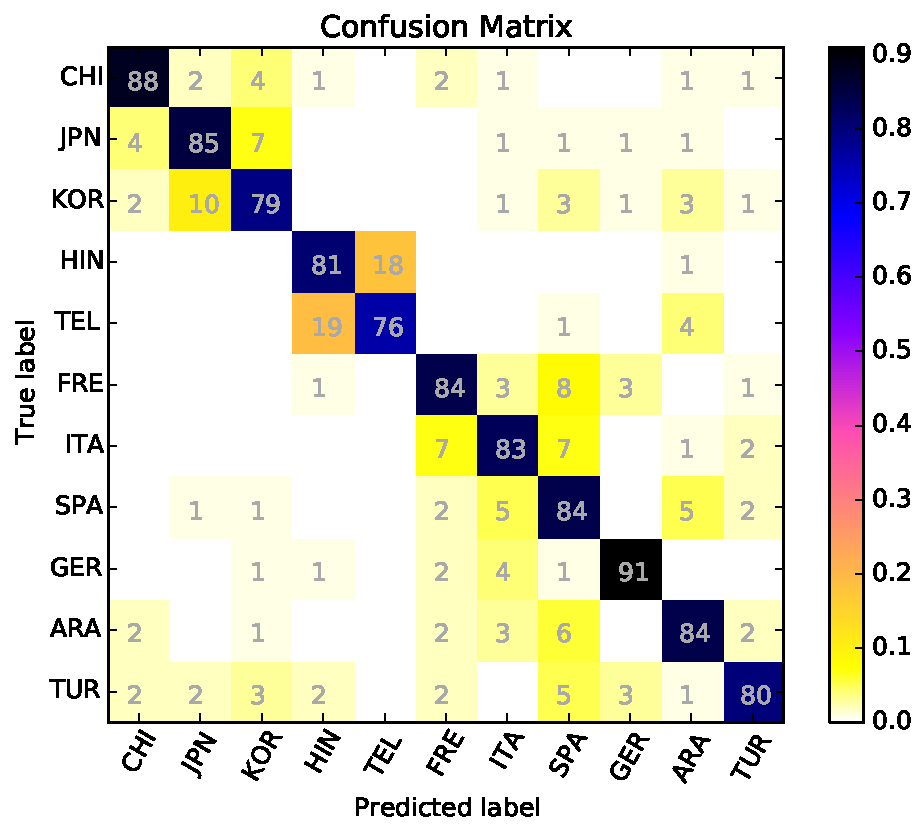
\includegraphics[width=0.7\textwidth]{closed_confusion_run06.pdf}
%TODO : add your own details to the caption for this figure
\caption{ESSAY track, closed training, bjerva 06 (ADD YOUR OWN DETAILS HERE)}
\label{fig:1}
\end{figure*}

\section{Analysis}

The ensemble seems to have overfit on the dev in most cases.


\section{Discussion}

\section{Conclusions}

\section*{Acknowledgments}

We wish to thank Noam Chomsky for inventing syntax.

\bibliography{bea12nli}
\bibliographystyle{emnlp_natbib}

\end{document}
